\documentclass[ignorenonframetext,]{beamer}
\setbeamertemplate{caption}[numbered]
\setbeamertemplate{caption label separator}{: }
\setbeamercolor{caption name}{fg=normal text.fg}
\beamertemplatenavigationsymbolsempty
\usepackage{lmodern}
\usepackage{amssymb,amsmath}
\usepackage{ifxetex,ifluatex}
\usepackage{fixltx2e} % provides \textsubscript
\ifnum 0\ifxetex 1\fi\ifluatex 1\fi=0 % if pdftex
  \usepackage[T1]{fontenc}
  \usepackage[utf8]{inputenc}
\else % if luatex or xelatex
  \ifxetex
    \usepackage{mathspec}
  \else
    \usepackage{fontspec}
  \fi
  \defaultfontfeatures{Ligatures=TeX,Scale=MatchLowercase}
\fi
\usetheme[]{Lumen}
% use upquote if available, for straight quotes in verbatim environments
\IfFileExists{upquote.sty}{\usepackage{upquote}}{}
% use microtype if available
\IfFileExists{microtype.sty}{%
\usepackage{microtype}
\UseMicrotypeSet[protrusion]{basicmath} % disable protrusion for tt fonts
}{}
\newif\ifbibliography
\hypersetup{
            pdftitle={Hey Hollywood, Where are the Women?},
            pdfauthor={Vatsala Ramanan, Margaret Bassney, and Emma Kornberg},
            pdfborder={0 0 0},
            breaklinks=true}
\urlstyle{same}  % don't use monospace font for urls
\usepackage{graphicx,grffile}
\makeatletter
\def\maxwidth{\ifdim\Gin@nat@width>\linewidth\linewidth\else\Gin@nat@width\fi}
\def\maxheight{\ifdim\Gin@nat@height>\textheight0.8\textheight\else\Gin@nat@height\fi}
\makeatother
% Scale images if necessary, so that they will not overflow the page
% margins by default, and it is still possible to overwrite the defaults
% using explicit options in \includegraphics[width, height, ...]{}
\setkeys{Gin}{width=\maxwidth,height=\maxheight,keepaspectratio}

% Prevent slide breaks in the middle of a paragraph:
\widowpenalties 1 10000
\raggedbottom

\AtBeginPart{
  \let\insertpartnumber\relax
  \let\partname\relax
  \frame{\partpage}
}
\AtBeginSection{
  \ifbibliography
  \else
    \let\insertsectionnumber\relax
    \let\sectionname\relax
    \frame{\sectionpage}
  \fi
}
\AtBeginSubsection{
  \let\insertsubsectionnumber\relax
  \let\subsectionname\relax
  \frame{\subsectionpage}
}

\setlength{\parindent}{0pt}
\setlength{\parskip}{6pt plus 2pt minus 1pt}
\setlength{\emergencystretch}{3em}  % prevent overfull lines
\providecommand{\tightlist}{%
  \setlength{\itemsep}{0pt}\setlength{\parskip}{0pt}}
\setcounter{secnumdepth}{0}

\title{Hey Hollywood, Where are the Women?}
\author{Vatsala Ramanan, Margaret Bassney, and Emma Kornberg}
\date{}

\begin{document}
\frame{\titlepage}

\begin{frame}

Date: May 4, 2019

\begin{figure}
\centering
\includegraphics{https://cdn1.thr.com/sites/default/files/imagecache/list_landscape_960x541/2016/12/39a_characters_01_flat-h_2016.jpg}
\caption{}
\end{figure}

In the past twenty years, women in the United States have made great
strides towards equality and representation. In 2007, Representative
Nancy Pelosi became the first female speaker of the House, while in
2016, Hillary Clinton became the first female presidential candidate
nominated by a major political party. In 2009, the Lilly Ledbetter Fair
Pay Restoration Act helped women file government complaints for pay
discrimination, and in 2013, women first entered combat positions in the
U.S. military. With all these monumental successes, one would expect a
reflection of this with positive female representation in popular media
and increased appreciation for such forms of entertainment. Does this
hold true in reality?

Let us consider the top ten PG-13 rated movies produced in the years
2000, 2008 and 2016, from the
\href{https://www.imdb.com/pressroom/about/}{Internet Movie Database},
or the imdb. Given that media representation most affects young,
developing minds, PG-13 rated movies are integral to this investigation
as their target audience, middle school-aged teenagers, are beginning to
explore their sexuality and identity. With this, female representation
in popular media is deeply influential in the {[}development of the
sense of self{]}
(\url{https://www.huffpost.com/entry/why-on-screen-representation-matters_n_58aeae96e4b01406012fe49d}).
Furthermore, the way women are represented in these movies affects how
young females view themselves and how young males view them, bringing
the issue into the real world. As we examine today's media
representation and its change over time, the three years of focus are
key because they are each roughly a generation apart, and can thus help
assess the progress made.

\end{frame}

\begin{frame}{How do we know if a movie truly represents women?}

Female representation is a rather subject concept. So, to determine
whether movies portray women with substantial importance, we refer to
the
\href{www.dailydot.com/parsec/fandom/mako-mori-test-bechdel-pacific-rim/}{Mako
Mori Test}. Named after a Pacific Rim character, the Mako Mori test
proposes an alternative to the popular Bechdel test. This test focuses
not on women conversing with each other as the Bechdel test does, but on
the story of at least one woman. The rules of the test are that (1) the
movie must have at least one female character, (2) that character must
get her own narrative arc, and (3) the arc cannot be dependent on the
man's story. While people still argue over whether or not ``Pacific
Rim'' was feminist or not, the test has great potential. For example,
Emma Stone's character from the 2016 movie La La Land passes the test as
she has an independent narrative arc which focuses on her ambitions to
be an actor. Here's a scene from the movie showing this:

However, the movie O Brother Where Art Thou? fails the test. As shown in
the scene below, the women do nothing more than seduce the male
protagonists of the movie and do not have independent goals and aims. In
this, the great actress Holly Hunter plays Penny, a character who is
seen as property by the male character Everett.

\end{frame}

\begin{frame}{What does the data tell us?}

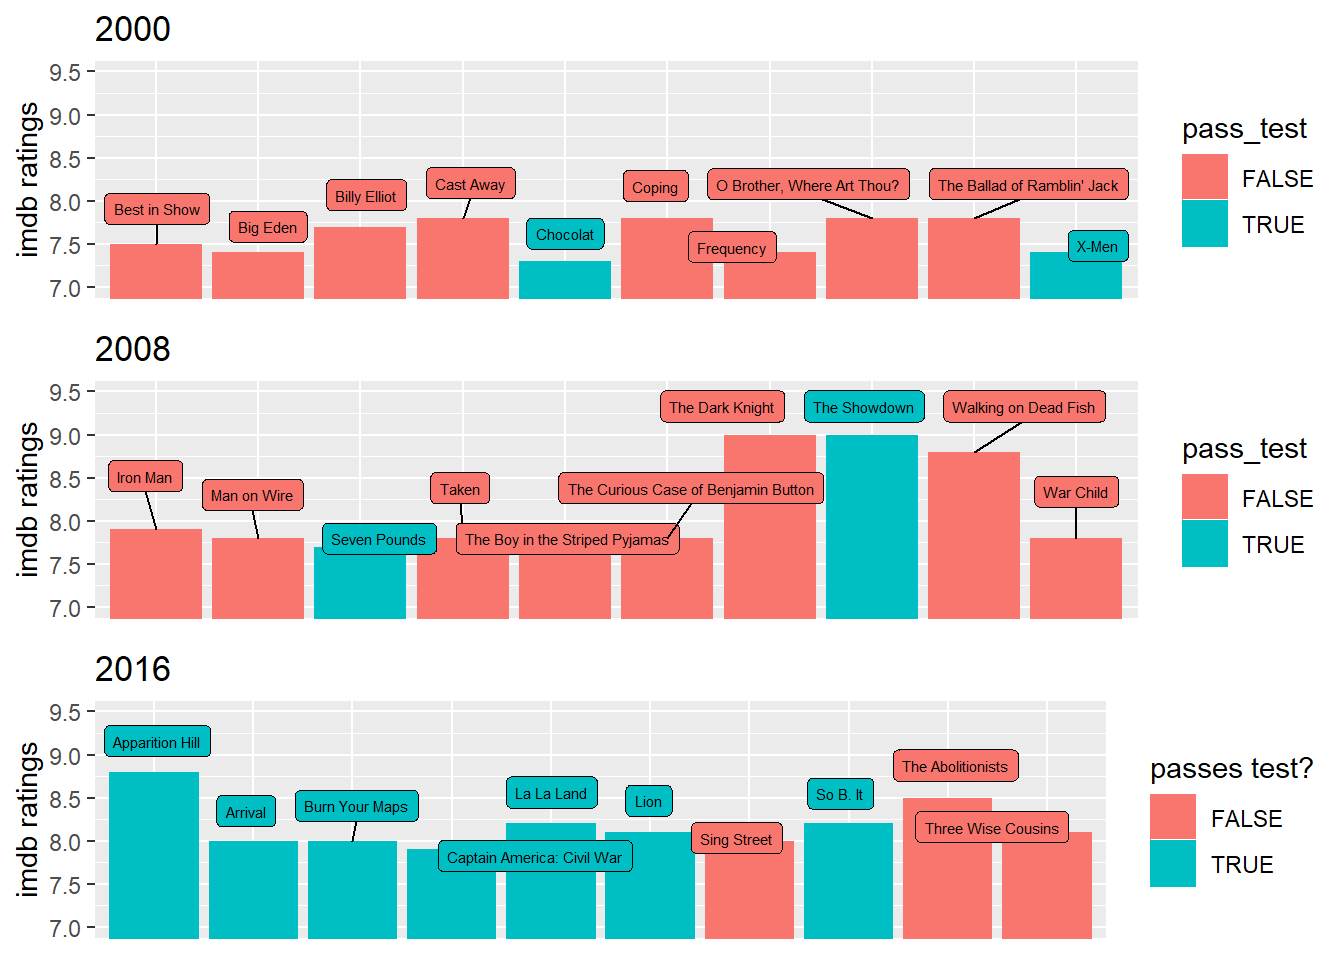
\includegraphics{sds192_miniproject4_files/figure-beamer/unnamed-chunk-8-1.pdf}

According to the imdb data, the early 2000's were not the kindest years
for women with the media representation of the time. In the year 2000,
the few top ten movies that do portray female representation are the
lowest rated. Every other top ten movie that year is male focused and
depicts women as objects.

However, eight years later, female representation begins to improve, if
marginally. In 2008, The Showdown is one of two films that passes the
test that year. It shares equal ratings with The Dark Knight, another
2008 film that does not pass the test. The only other movie that year to
pass the test was Seven Pounds and it experienced the lowest ratings
among the top ten movies.

Finally, another eight years later, the representation of women improves
dramatically. In 2016, not only do the majority of the top ten IMDB
rated movies pass the test, but these movies are also the movies with
the highest ratings. While the majority of the 2008 movies that failed
the test were violent, in 2016, the majority of the movies that did pass
the test were nonviolent.

At this point, we must take into account that how we interpret our data
may be influenced by the fact that, as time goes on, technology
advances. With this, higher quality movies are being produced and, in
turn, ratings increase. Thus, past movies with positive representation
of women may not have been been rated as highly due to the lower
production quality.

One interesting thing to note is the fact that the movies in 2016 that
show positive female representation, score higher than the top rated
movies of 2000 which did not have good representation. This could be
explained by the fact that good women characters make movies better but
it could also be true that the production value is just higher. For
example, in 2000, no movies score higher than 7.8 but in 2016, all of
the movies that pass the test score 7.9 or higher. Only two movies in
2008 score higher than 7.9. The movie ``The Showdown'' scored 9.0 and
the movie ``Seven Pounds'' scored 7.7. This means 50\% of the movies
that passed the test in 2008 scored fairly high. The percentage of the
movies that didnt pass the test in 2008 that scored high ratings is only
25\%.

Although we see the representation of women rise in 2016, progress is
still necessary. With every movie we examined, men were always
positively represented. This shows that it is possible to consistently
positively represent one gender identity and means that it can and
should be done for woman as well.

\end{frame}

\end{document}
